\chapter{Experiments}\label{ch:experiments}
In order to get the limits and the usability of the tools in table \ref{table:tools} for high bandwidth session based throughput testing, the tools are used in various experiments.
The results the research is looking for is: 
\begin{itemize}
\item{The capability of generating 40Gb/s of bandwidth} 
\item{The maximum amount of packets per second} 
\item{The maximum amount of sessions per second the tools are capable of opening}
\end{itemize}

The 'easy to use tools' are tested on top of two different kernels. 
FreeBSD 11.0 and Ubuntu 16.04 are used to see if the kernel has any influence on one of the three bullet points.
The reason for the two kernels is that a preliminary test showed major differences in generating an amount of UDP packets per second.  
The DPDK tools are tested on top of the Ubuntu kernel since FreeBSD does not support DPDK.
All experiments described in this chapter are executed in a test environment at Nikhef. The simplified visualization of the test environment is displayed in figure \ref{fig:testenv}. \\ 

\begin{figure}[H]
  \includegraphics[scale=0.45]{images/testenv.pdf}
  \caption{Used environment for experiments.}
  \label{fig:testenv}
\end{figure}

The figure shows five server systems, of which three identical servers (A, B and C in table \ref{tab:testmachines}) are used to perform the tests whose results are described in this paper.
During the experiments 2 extra machines (D and E in table 4.1), both containing 100Gb/s Mellanox cards, have been introduced in the network to test links with a capacity up to 100Gb/s and to verify if reached limits are resource or hardware based. All servers were connected to a Juniper QFX10002 (device S in Fig. \ref{fig:testenv}), which provides 32 40Gb/s QSFP ports, of which some can be and are configured as a single 100Gb/s interface.

\begin{table}[H]
\centering
\caption{Specifications from the machines used for experiments}
\label{tab:testmachines}
\begin{tabular}{|l|l|l|l|}
\hline
\textbf{Machine} & \textbf{A \& B \& C}                                                                          & \textbf{D}                                                                                    &\textbf{E}                                                                     \\ \hline \hline
Threads & 8                                                                                    & 56                                                                                   & 128                                                                   \\ \hline
CPU     & \begin{tabular}[c]{@{}l@{}}Intel(R) Xeon(R) CPU \\ E3-1230 v5 @ 3.40GHz\end{tabular} & \begin{tabular}[c]{@{}l@{}}Intel(R) Xeon(R) CPU \\ E5-2697 v3 @ 2.60GHz\end{tabular} & POWER8E                                                               \\ \hline
Memory  & 4x 16GB @ 2133 Mhz                                                                   & 24x 8GB @ 1067Mhz                                                                    & 2x 64GB                                                          \\ \hline
NIC     & \begin{tabular}[c]{@{}l@{}}Intel XL710 \\ 40Gb/s\end{tabular}                        & \begin{tabular}[c]{@{}l@{}}Mellanox ConnectX-4\\ 100Gb/s\end{tabular}                & \begin{tabular}[c]{@{}l@{}}Mellanox ConnectX-4\\ 100Gb/s\end{tabular} \\ \hline
\end{tabular}
\end{table}

Device A is always acting as the destination for traffic unless stated otherwise. Depending on the tests the source can be machine B, C or B and C together.
This depends on the capability of the tools tested at that moment.
For testing beyond 40Gb/s, one of the 100Gb/s machines (D or E) can be used.
Machine M is a Simple Network Management Protocol (SNMP) collector. This SNMP collector query's the test servers every 10 seconds for status. 
Packets per second and bits per second are retrieved from the devices under test.
Switch S is also added to the collector as a data source. 
SNMP is active on the management interface of the devices.
The high bandwidth interfaces are able to connect to each other over a non-routed VLAN. This makes sure the test traffic cannot interfere with SNMP reads from collector M. 

\section{Standards and best practices}\label{sub:rfc}
Multiple RFC's have been written that provide guidelines for throughput testing.
The terminology from RFC 1242\cite{rfc1242} will be used throughout this paper and techniques from RFC 2544 \cite{rfc2544} have been taken into account during this research.
However, the aforementioned practices and benchmarks of RFC 2522 (and 6349\cite{rfc6349}) are centered on traffic generation that overloads network devices, which is detrimental to user network experience in production (shared) networks, as was discussed in RFC 6815\cite{rfc6815}.

A quick list with guidelines from these RFC's is as follows:

\begin{itemize}
\item{Throughput tests should have a minimum runtime of 60 seconds}
\item{The environment cannot be a production environment}
\item{Devices under test (DUT) will possibly be overloaded}
\item{Tests should be done 3 times and averages taken from the results.}
\end{itemize} 

\section{'Easy to use' tools}
Tools that require a command line argument to start generating load using the kernels drivers and resources are marked as 'easy to use' tools for this report.  
All the 'easy to use' tools are tested running on top of Ubuntu and FreeBSD.
All the tools where used to finds its limits for bandwidth generation, maximum amount of pps and maximum amount of sessions.

\paragraph{iPerf3}\mbox{}\\
Machine A is set up as a server running on default TCP port 5201, machine B is setup as a client connecting to the server. 
Tests are executed from the client side on a FreeBSD and Ubuntu server , the performance differences where minimal. 
The initial tests were performed sending 64 bytes of traffic in each packet. The practical maximum amount of packets (42Mpps) was not reached until 6 threads where used to generate traffic (the practical maximum amount of packets is explained in section \ref{sub:pktgen}). 
The links capacity was filled using 16 threads and a packetsize of 1500 bytes. 
iPerf3 start a TCP session per running thread, this makes it less useful for this project since we explained that only bandwidth is not enough to reach performance limits when one is looking to overload a device.

\paragraph{Hping}\mbox{}\\
Hping is used to send spoofed traffic to a server. 
It does not need a server side application running on server A. Therefore only the client side was tested on top of FreeBSD and Ubuntu.
Both kernels where capable of sending a maximum of 13Gb/s of SYN packets towards a server padded up to 9000 bytes. Although it has nice features to craft packets and probably has the capacity to overload certain small environments, the maximum bandwidth is sub-par for this project.  

\paragraph{Bonesi}\mbox{}\\
The maximum output that was produced with BoNeSi was 300Mb/s and 500Kpps on a Ubuntu machine. 
But not much difference is found during the tests between the two different kernels.
The reached limits are not sufficient for this project and therefore BoNeSi will not be used for further experiments. 

\section{Tools using the Data Plane Development Kit}
The Data Plane Development Kit (DPDK) enables fast packet generation and transportation inside a system. Tools are available to generate packets of RAW UDP and RAW TCP data. A recent tool is introduced that offers HTTP v1.1 packet generation. The tools tested during these experiments are: pktgen, MoonGen and WARP. 

\subsection{pktgen}\label{sub:pktgen}
For this experiment, like all others, server A is the destination for the generated traffic, server B is the source which is generating the traffic. 
Both machines are identical as seen in table \ref{tab:testmachines}. Pktgen is not a client server based application. 
System A is idle, B will generate traffic in the form of SYN packets. 
To find the hardware limitations one can send small packets of 64 bytes which should show the hardwares capabilities of generating packets or one should generate larger packets of 1500 bytes (not considering jumbo frames) to fill up a links capacity.\\
 
When sending small packaged to the destination the maximum amount of packets per second peaked at 42Mpps where the expected amount of packets is 56Mpps unidirectional. 
Additional configuration was therefore carried out in order to ascertain the cause of this 42Mpps limit. 
The DPDK website offers a guide \cite{intelguidedpdk} to setup the system in order to get the maximum performance out of the Intel XL710 40Gb/s card. 
Flashing a new firmware version into the card was a first step. 
After following the DPDK guide the result remained the same. 
According to conclusions drawn out of a report from Chelsio \cite{chelsio} the PCI express bus (V3.0, 8.0GT/s, 8 lane) is capable of transferring 70Mpps bidirectional. 
Unidirectional it can reach a maximum of 42Mpps.
Both the Chelsio\cite{t580} and the Intel\cite{xl710} card use the PCIe v3.0 (8.0 GT/s) 8 lane interface to connect to the main board.
The limitation caused by the PCI express bus gives the research a new practical maximum amount of pps (42 million) transferred by a host.
   
Ramping up the packet size, starting at 64 bytes and adding 16 bytes per test round up to a maximum of 1024 bytes, resulted in finding the optimal packet size of 400 bytes. 
This generated a bandwidth usage of 39.8Gb/s and a total of 11Mpps. Figures \ref{fig:pktgenlink} and \ref{fig:pktgenpps} display the amount of bandwidth transferred and the amount of pps transferred during a tests using 400 byte packets. 

\begin{figure}
  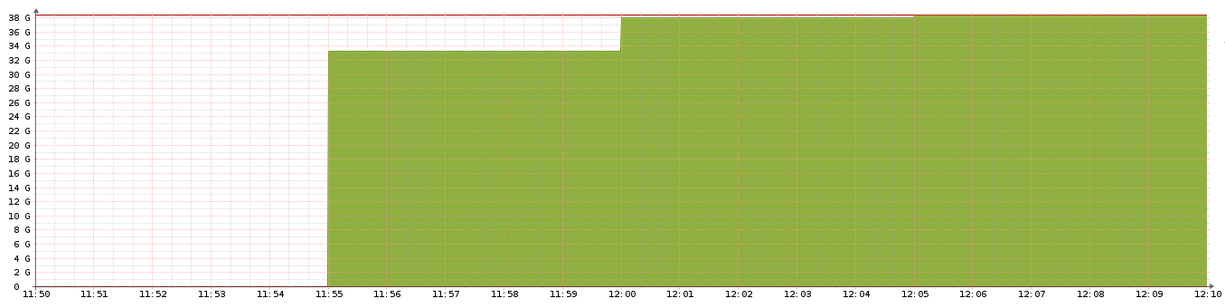
\includegraphics[scale=0.35]{images/pktgen_link_usage.png}
  \caption{Pktgen link usage for 400 byte packets (generated bandwidth at time x, graph displays an average of used bandwidth over 5 minutes}
  \label{fig:pktgenlink}
\end{figure}

\begin{figure}
  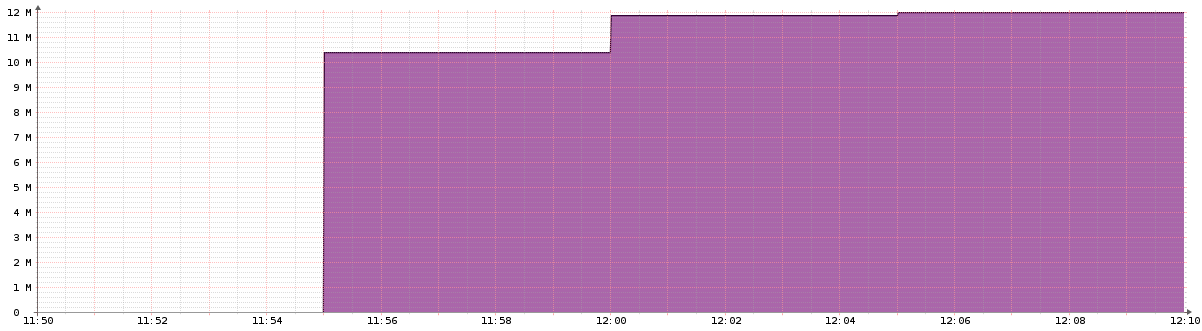
\includegraphics[scale=0.35]{images/pktgen_pps.png}
  \caption{Pktgen packets per second for 400 byte packets (generated packets per second at time x, graph displays the average transported pps over 5 minutes}
  \label{fig:pktgenpps}
\end{figure}

\newpage

\subsection{WARP}\label{sub:warp}

A WARP client needs a service to respond to SYN packets, otherwise sessions are not opened up and there will be no traffic flowing. 
To find the capabilities of WARP on the servers available in the test environment a benchmark was run on server B. 
Appendix \ref{appendix:software} displays the benchmark used for this test. 
An extra Intel XL710 card is added to machine B since the XL710 cardi can not utilize both NIC's in one slot at their full capacity.
The second NIC is designed as a fail over interface. 
NIC A from card 1 is connected to switch S, NIC A from card 2 is also connected to switch S. 
All the CPU's and all the memory will be dedicated for this test. 
The benchmark first does the tests for RAW TCP, where after it will perform the tests using HTTP v1.1.

During both tests 4 million sessions are the goal.
The client side of the benchmark tries to open 4 million session, not all of them succeed. The time spend for all the sessions to succeed or to time-out is measured.
The goal for this test is to find the capabilities of the server while it is running WARP therefore RFC2544 is not applicable 

The first test is RAW TCP. As seen in figure \ref{fig:rawtcpsession} about one million sessions per second are tried to open by the client.
The succeeded sessions use up some of the links total capacity as is displayed in figure \ref{fig:rawtcplink}.  

\begin{figure}[H]
  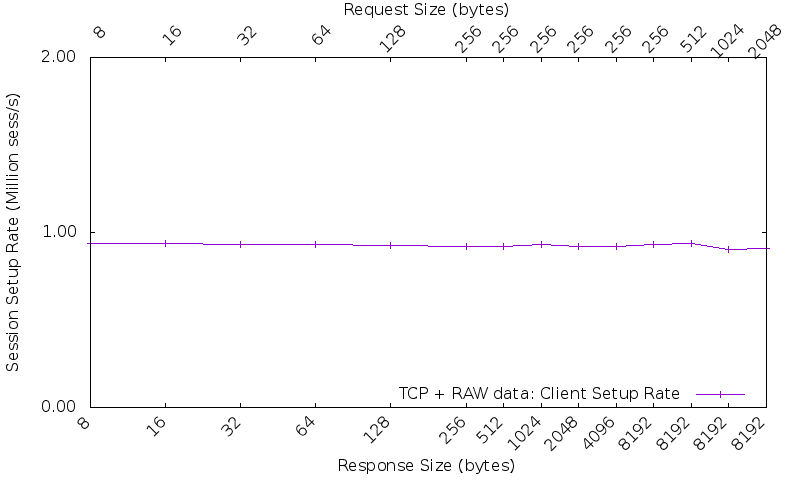
\includegraphics[scale=0.6]{images/raw_setup.png}
  \caption{Amount of requested session per second from the client to the server for raw TCP (amount of requested sessions versus the request(Rx) and respond(Tx) size)}
  \label{fig:rawtcpsession}
\end{figure}

\begin{figure}[H]
  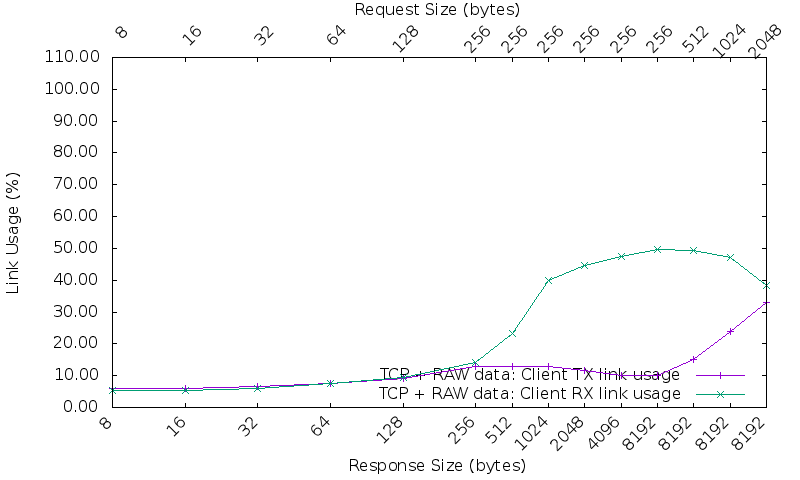
\includegraphics[scale=0.6]{images/raw_link_usage.png}
  \caption{Link usage for raw TCP (percentage of link usage versus the request(Rx) and response(Tx) size)}
  \label{fig:rawtcplink}
\end{figure}

The second test contains a HTTP file request. The server responds with a 200-(OK) message using a configured file size.
The server was able to generate around one million sessions per second as seen in figure \ref{fig:httpsession}. Where not all of the sessions where answered in time.
Figure \ref{fig:httplink} shows the bandwidth usage for HTTP traffic for the established sessions. 

\begin{figure}[H]
  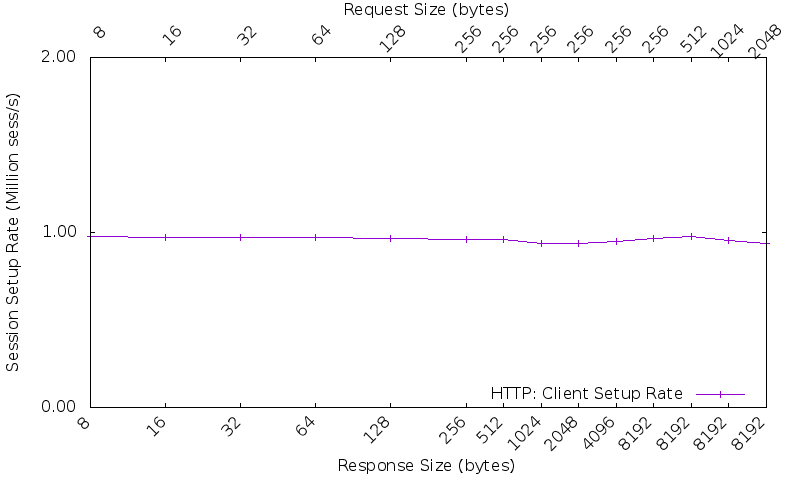
\includegraphics[scale=0.6]{images/http_setup.png}
  \caption{Amount of requested sessions per second from the client to the server for HTTP (amount of requested sessions versus the request(Rx) and respond(Tx) size)}
  \label{fig:httpsession}
\end{figure}

\begin{figure}[H]
  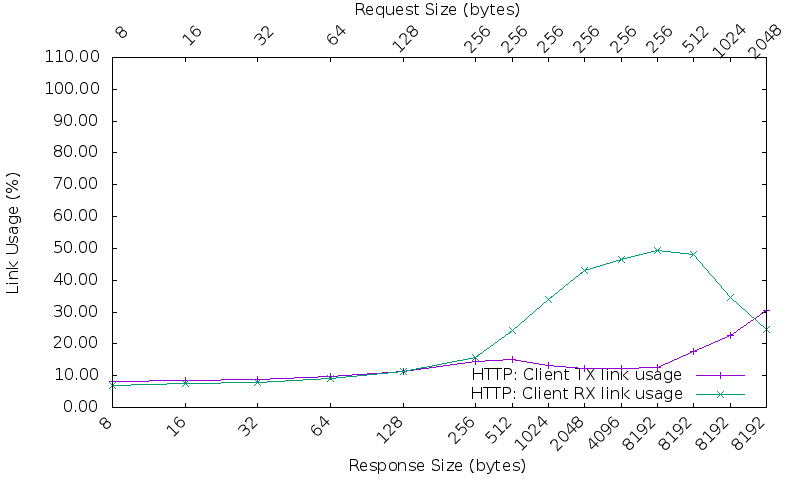
\includegraphics[scale=0.6]{images/http_link_usage.png}
  \caption{link usage for established sessions at HTTP  (percentage of link usage versus the request(Rx) and response(Tx) size)}
  \label{fig:httplink}
\end{figure}

From the figures we can see WARP is capable is generating 1 million sessions per second and can fill up half of the links capacity when large packets are generated.
This makes WARP very interesting to use for application level testing purposes. 

\subsection{MoonGen}
MoonGen offers benchmark scripts to determine the machines capabilities. 
The benchmark script used for the tests can be found in appendix \ref{appendix:software}. 
A single machine (B) is connected to the switch using two 40Gb/s NIC's at 2 separate cards (similar to the setup of the WARP test), both connected to switch S (one NIC for the server part and the other for the clients part of the benchmark). Sending UDP traffic with a size of 1500 bytes resulted in a maximum of 24 Gb/s. When the smallest possible Ethernet packets of 64 bytes are send over the line a maximum of 15Mpps is reached. When TCP is used on the same machine (B) connected to the switch using two interfaces, a maximum of 10Gb/s was reached. These low values did not make MoonGen interesting enough since Pktgen is capable of reaching hardware limits. 


